\section{Towards a User-Centered Attestation}

Instead of defining yet another Trusted Virtualized Platform, the following subsections will explore what sort of properties and operations can lead to the conclusion that a particular platform can be \emph{trusted}.

\subsection{Principles of Remote Attestation}

The need for remote attestation and its process have been defined by the TCG~\cite{VTPA,ISOTPM}. However, besides the basic interaction with the TPM, which can be summarized as a trustworthy mechanism, an attestation should follow general principles outlined by\cite{RA}: 

\begin{prince}\label{pri:1} Fresh information. Information about the target of an attestation should reflect the running system, e.g. programs it is currently running and not just disk images. The reasoning is that showing only disk images tells very little about which part of this configuration is actually running. Inspired by measurement tools that provide merely measured boot, i.e. a boot sequence that reports the disk contents in the form of a hash will not supply information as to whether or not any (protection) mechanisms available on disk are actually being executed. Other measurement tools provide \emph{load-time} information by reporting hashes of executed binaries, while in more recent years approaches for measuring active memory have emerged. An appraiser may, however, have its own expectations as to how \emph{fresh} the evidence is which leads to the next principle. 
\end{prince}

\begin{prince}\label{pri:2} Comprehensive information. An attestation mechanism should be capable of delivering comprehensive information. This implies that such an attestation mechanism must have access to all internal states and must be able to report these using local measurement tools. While this inevitably leads to concerns about \emph{dangerous} disclosure, i.e. reporting vulnerable states, and ultimately raises privacy questions, it also \emph{should} consider a problem related to the amount of reference measurements in an appraisers' database --- especially if there aren't any specialized appraisers.
\end{prince}

\begin{prince}\label{pri:3} Constrained disclosure. An attestation target should be able to decide which information is sent to a particular appraiser. The appraiser should be identifiable and the target platform must be able to enforce policies defining what evidence it supplies to an appraiser. Rather than suggesting the appraiser to be identifiable, it should be suggested that the appraiser reveals the type or amount of evidence it \emph{requires} in order to be convinced. This implies that there is a semantic for attestations which leads to a conclusion as to whether or not a target can be trusted.  
\end{prince}

\begin{prince}\label{pri:4} Semantic explicitness. The semantics of an appraisers' trust decision should be explicitly defined in logic. As an example on a local scale, it should define that a trust decision is made about a particular service, or the entire target platform and how trust in a particular service is established by supplying evidence of supporting or coexisting services on the target. Furthermore, it must be defined how subsequent attestations affect the initial decision and how they can be correlated for logical inferences. 
\end{prince}

\begin{prince}\label{pri:5} Trustworthy mechanism. Appraisers need to infer the trustworthiness of the mechanism that is used to deliver evidence to them. This principle, although introduced last, is intuitively critical as not fulfilling it invalidates all principles so far since the evidence might simply not be convincing as it can not be trusted. 
\end{prince}

These principles were defined as general requirements for attestation architectures utilizing a trustworthy mechanism to supply convincing evidence about a particular platform. However, w.r.t. virtualization and in an Network Functions Virtualization (NFV) scenario Lauer et al.~\cite{lauer2016} have extended these principles to address issues related to the multi-user and multi-layer architecture of virtualized environments:

\begin{prince}\label{pri:6} Layer linking. When a virtual environment is attested, its underlying components or layers must also be attested. Attesting a virtual platform without inspecting its underlying layers and ultimately the physical platform supplies only very limited evidence to an appraiser making a trust decision. A quote generated by a virtual trust agent such as the vTPM must be substantiated by a TPM quote so as to indicate the trustworthiness of the virtual trust agent's quote. 
\end{prince}

\begin{prince}\label{pri:7} Scalability. Since attestation, i.e. (v)TPM quotes, can occur for any virtual machine triggered by any user or appraiser, substantiating each vTPM quote with a TPM quote will inevitably lead to the TPM becoming a bottleneck in a virtualization scenario. An attestation mechanism must treat the TPM as a limited and shared resource and offer a scalable protocol between vTPM and TPM quotes.  
\end{prince}

Principles~\ref{pri:6},~\ref{pri:7} can be seen as a virtualization specific addition to principle \ref{pri:5}. Following these principles also reveals the proposition of this paper: Using a trustworthy mechanism implies that all other principles apply to the trustworthy mechanism itself.

\subsection{Attestation in Virtualized Environments}

Following these principles, two distinct approaches (or variants) have emerged in research and current standardization work. The first approach being a direct translation of remote attestation protocols using the vTPM associated with a VM as the key component of the trustworthy mechanism in combination with an attestation of lower layers using the same protocol but this time with the TPM. The later approach~\cite{lauer2016} was introduced subsequently as a solution for NFV and \emph{X-as-a-Service} infrastructure. It assumes multiple VMs and \emph{few} or no VM users and a single hypervisor operator. The trustworthy mechanism relies solely on the TPM while vTPMs are utilized as potentially untrusted sinks for upper layer measurements. The following paragraphs will detail these two approaches based on the principles~\ref{pri:1}-\ref{pri:7}.  

\subsubsection{Attestation Approach I}

Attestation approach I attests virtual and physical environments using the \emph{same} attestation mechanism (Fig. \ref{fig:type1attest}). An approach treating VM and lower layers equally has intuitive benefits: it is easy to integrate in an existing protocol landscape~\cite{DAA,ISOTPM}, architectures implement vTPMs as virtual devices\cite{vtpm,lauer2016}, appraisers can reach a trust decision using a \emph{standard} evaluation of the evidence or include the properties of layered systems dynamically.

\begin{figure}[!ht]
  \centering
    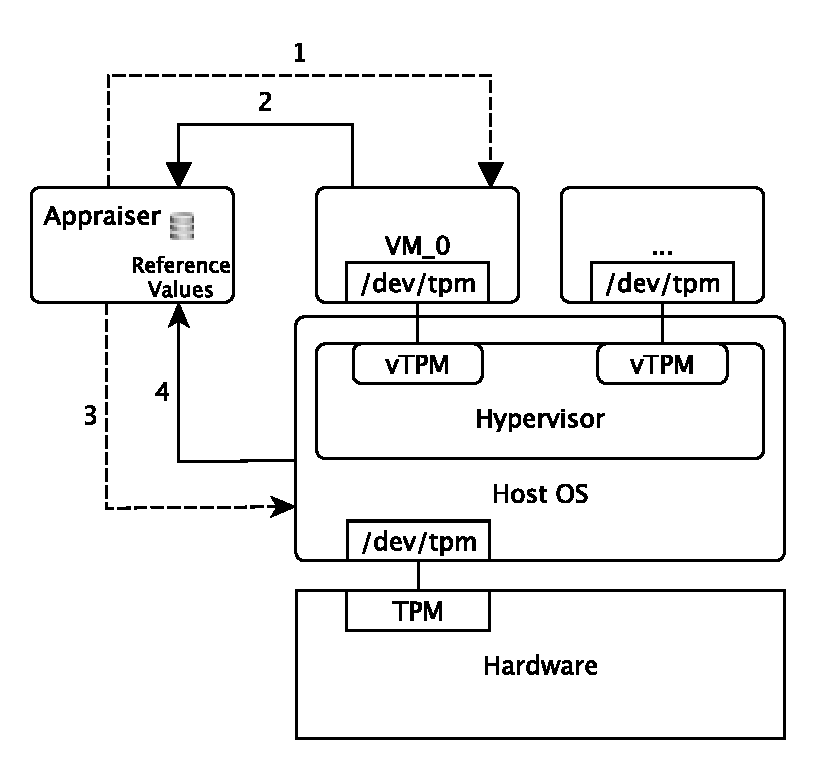
\includegraphics[scale=0.35]{figures/type1attest.pdf}
  \caption{Attestation Approach I illustrated. The appraiser, holding \emph{suitable} reference values, requests evidence from different layers sequentially. Boxes denote hardware modules, rounded containers denote attestable software components. Dashed lines indicate requests for meta data and bold lines indicate evidence responses.}
  \label{fig:type1attest}
\end{figure}
\begin{table}
  \caption{Fulfillment of attestation principles in a system using separate VM - hypervisor attestations.}
\label{tab:1}
  \centering
\begin{tabular}{p{1cm}|p{(\hsize / 3) * 2}} %6.5 plus whatever seems to fill two column
 \toprule
 Principle & Fulfillment \\ \midrule
 % Fresh information
 \ref{pri:1} & Requires measured or trusted boot, can accommodate Integrity Measurement Architecture (IMA)~\cite{IMA} for load time measurements of binaries.\\
 \midrule
 % Comprehensive information
 \ref{pri:2} & During boot each component measures its successor into a PCR. As soon as the kernel is measured and loaded, the kernel load mechanism is responsible for measuring newly loaded binaries. \\ 
 \midrule
 % Constrained disclosure
 \ref{pri:3} & Appraisers do not have to be known to the target, mutual attestation is not part of any proposal. \\
 \midrule
 % Semantic explicitness
 \ref{pri:4} & The trust decision is based on whether or not supplied evidence as hash values of binaries can be found in a reference database. The appraiser then correlates attestations of any layer $n$ with layer $n-1$. An appraisal of a VM depends on the appraisal of its hypervisor. \\
 \midrule
 % Trustworthy mechanism
 \ref{pri:5} & The trustworthy mechanism includes a TPM quote over a PCR (along with IMA log for hash verification) for the hypervisor. The attestation process is completed through a vTPM quote over vTPM PCRs and respective logs explaining the platform configuration hash. Credentials in a vTPM must be \emph{trustworthy} and protected from leakage. \\
 \midrule
 % Layer linking 
 \ref{pri:6} & The appraiser must have \emph{a priori} information about the locality of a VM or a list of VMs hosted by an hypervisor, a VM - hypervisor mapping. Assuming integrity and availability for such a mapping, the appraiser can correlate TPM and vTPM quotes when evaluating evidence in a decision process. \\
 \midrule
 % Scalability 
 \ref{pri:7} & 1:1 relation between TPM and vTPM quotes assuming each vTPM quote must be preceded or succeeded by a TPM quote (depending on principle~\ref{pri:4},\ref{pri:5}). \\
 \bottomrule
\end{tabular}
\end{table}

\emph{Discussion.} Separate attestation approaches are favorable for an implementer as they require little modification to existing trust establishment processes. However, this also implies specific assumptions towards the entire attestation system. Principles~\ref{pri:1},~\ref{pri:2} are fulfilled using what is the \emph{de-facto} standard in Trusted Computing approaches for accessing and measuring components for later evaluation by an appraiser. In a virtualized scenario, it should be noted that it is the hypervisors responsibility to maintain necessary components such as the vTPM as a root of trust for storage while the VM configuration must supply boot code that acts as the root of trust for measurement. Principle~\ref{pri:4} and~\ref{pri:5} are closely related and demand a rigorous definition of trust, especially, concerning the correlation of the two kinds of measurements. Explicit semantics of a trust decision are critical for a protocol design and evaluation and the traditional approach of matching well-known hashed to measured hashes is not suitable for comprehensive decisions. As far as the trustworthy mechanism is concerned, the presented approach relies on a critical assumption: VMs and associated vTPMs are not only strongly coupled but also isolated. Since the vTPM is required to perform \emph{quotes} over its Platform Configuration Registers (PCRs), credentials must only be accessible to authorized parties such as the VM itself. However, even under the assumption of \emph{strong} isolation, the underlying hypervisor still has responsibilities which, in an effort to provide comprehensive information, must also be reviewed. Consequently, a VM attestation must be followed by an attestation of the hypervisor --- or vice versa? Intuitively, causality dictates that the hypervisor provides the run-time for a VM and therefore any property of the hypervisor affects the trustworthiness of the VM: attesting the hypervisor and subsequently attesting the VM seems effective. However, another interpretation would be that the appraisal of a VM becomes \emph{effective} only after the hypervisor has been attested. Both interpretations seem to fulfill the attestation requirement in prose which again emphasizes the need for clear semantics.


\subsubsection{Attestation Approach II}

The second approach towards attestation of virtual machines is distinctly different from separate, legacy attestations insofar as it is intended for virtualized infrastructure such as \emph{X-as-a-service} and NFV. Entitled ``Hypervisor-based Attestation'', the approach relies solely on the TPM and mechanisms recorded into PCRs to collect and supply evidence to an appraiser --- this implies that even the \emph{trustworthy mechanism} can be verified. The vTPM itself does not need to perform a quote over internal data structures and therefore, with attestation in mind, does not need to be raised to a \emph{somewhat} trusted level. The attestation flow is outlined in Fig. \ref{fig:type3attest}.

\begin{figure}[!ht]
  \centering
  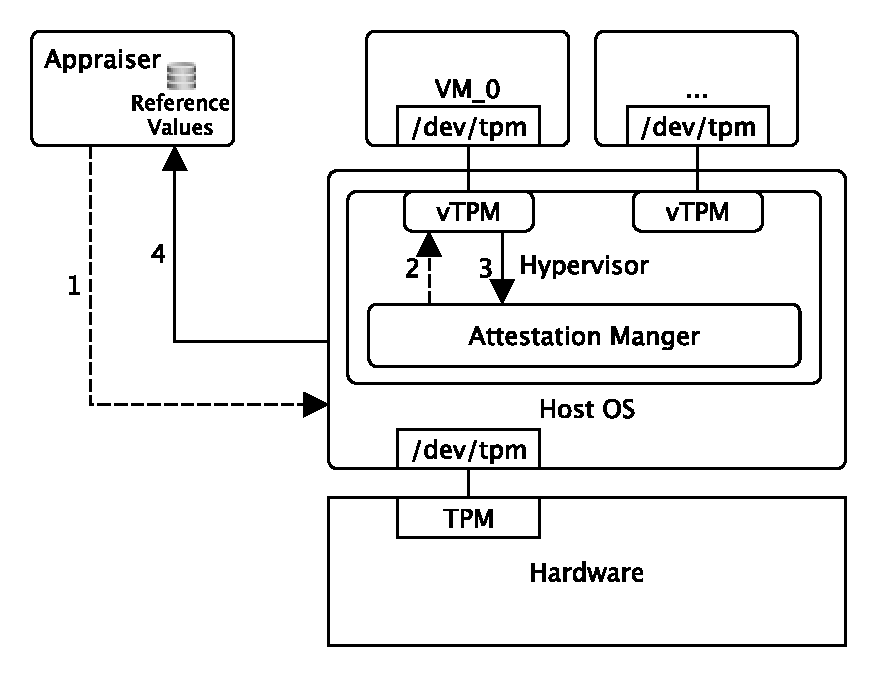
\includegraphics[scale=0.35]{figures/type3attest.pdf}
  \caption{Hypervisor-based Attestation. The Appraiser attests the Target including \emph{n}-VMs. Attestation Manager, a process in the Host OS or hypervisor, collects individual evidence produced by VMs from a vTPM interface. Subsequently, the attestation target sends a response containing its own and each VMs evidence.}
  \label{fig:type3attest}
\end{figure}

\begin{table}
\caption{Fulfillment of attestation principles in a system using hypervisor-based attestations.}
\label{tab:2}
\centering
\begin{tabular}{p{1cm}|p{(\columnwidth / 3) * 2}} %6.5 plus whatever seems to fill two column thingy nicely
 \toprule
 Principle & Fulfillment \\
 \midrule
 % Fresh information
 %\ref{pri:1} & Requires measured or trusted boot, can accommodate Integrity Measurement Architecture (IMA)~\cite{IMA} for load time measurements of binaries.\\
 \ref{pri:1} & Same as Table \ref{tab:1}.\\
 \midrule
 % Comprehensive information
 %\ref{pri:2} & Measurement tools are either pre-kernel or kernel based for all layers.\\
 \ref{pri:2} & Same as Table \ref{tab:1}.\\
 \midrule
 % Constrained disclosure
 %\ref{pri:3} & Appraisers do not have to be known to the target, mutual attestation is not part of any proposal. \\
 \ref{pri:3} & Same as Table \ref{tab:1}.\\
 
 \midrule
 % Semantic explicitness
 \ref{pri:4} & Supplied hash-logs are compared against \emph{golden values}, unknown values indicate untrustworthy states.\\
 \midrule
 % Trustworthy mechanism
 \ref{pri:5} & The trustworthy mechanism is comprised of a two stage measurement process. The first stage measures hypervisor components, including the attestation manager and vTPMs. The second stage measures VM components into vTPMs. For reporting, only the TPM is consulted and vTPM PCRs are collected and attached to a hypervisor attestation.\\
 \midrule
 % Layer linking 
 \ref{pri:6} & Once the appraiser has verified the attestation manager and vTPMs, the inspection of VM measurements reveals the hypervisor - VM mapping. Prior knowledge of VMs and hypervisor mappings is not required.\\
 \midrule
 % Scalability 
 \ref{pri:7} & 1:n relation between TPM and VM attestations. \\
 \bottomrule
\end{tabular}
\end{table}

\emph{Discussion. }Hypervisor-based attestation approaches (Fig. \ref{fig:type3attest}) have three common benefits: Bottom-up attestation, coupled hypervisor-VM attestations, and inherently \emph{en bloc} evaluation. Regarding the trustworthy mechanism (Principle \ref{pri:5}), a hypervisor-based, bottom-up attestation is, at a glance, uncontroversial and in-line with conventional attestation strategies. However, common approaches use IMA~\cite{IMA}, a kernel-based loader extension, exclusively once the module is loaded to measure and propagate loaded components to the TPM. An attestation manager or vTPM will, instead of reporting to the TPM, keep \emph{own} records - the integrity of this functionality is then appraised using the load time hash of these components. As a result, the trust that can be placed in the completeness and correctness of such records is transitive and relies on trusting supporting mechanisms such as the attestation manager and vTPM instance. In fulfillment of Principle~\ref{pri:4}, such considerations should be addressed by a defined trust decision process that includes and respects the concept of \emph{transitive} trust relationships. Furthermore, \cite{lauer2016} does not specify how individual VM appraisals affect trust decisions for other VMs running on the same platform --- a lack carried over from utilized measurement architectures.

\subsection{Observations}\label{subsec:observations}
Having revisited both attestation approaches, the following observations can be made: (i) Attestation of a layer inadvertently requires attestation of the layers below. (ii) Even if the Virtual Trusted Agent, or vTPM, is used for a signature, the trustworthiness of that signature relies on the appraisal of the hosting layer. (iii) Neither approach is semantically explicit with respect to their treatment of evidence in layered systems beyond suggesting exhaustive platform hash comparisons. (iv) Designated appraisers are present and capable of correlating and evaluating supplied evidence. (v) Most importantly, knowledge and connectivity of lower layers is assumed. 


